\documentclass[11pt]{article}
\usepackage{times,epsfig,subcaption,wrapfig,algorithmic,color,boxedminipage,graphicx,url}
\usepackage{authblk}
\setlength{\affilsep}{0em}
\usepackage{debulletin}
\usepackage{etoolbox, totcount}
\usepackage{import}
\usepackage{xcolor}
\usepackage{authblk}
\usepackage{microtype}
\usepackage{multirow,url,amsmath,amsfonts,amssymb,xspace}
\usepackage{hyperref}
\usepackage{balance}  % for  \balance command ON LAST PAGE  (only there!)
\usepackage{booktabs} % For formal tables
\usepackage{enumitem}
\usepackage{multirow}
\usepackage{subcaption}
\usepackage{authblk}
\usepackage{appendix}

% \usepackage[pdfpagelabels=false]{hyperref}

\usepackage{listings}

\usepackage{outlines}



%deepeye
\usepackage[lined,boxed,vlined,ruled,linesnumbered]{algorithm2e}
\DeclareMathAlphabet{\pazocal}{OMS}{zplm}{m}{n}
\DeclareMathOperator*{\argmax}{arg\,max}


% \newcommand\mycommfont[1]{\footnotesize\textit{ #1}}
% \SetCommentSty{mycommfont}


\usepackage[color,matrix,arrow,all]{xy}
\usepackage{tikz}
\usetikzlibrary{shapes,decorations}
\usetikzlibrary{calc}



\usepackage[english]{babel}
\usepackage[utf8]{inputenc}
\usepackage{enumitem,kantlipsum}
\usepackage{graphicx, color}
\usepackage{wrapfig}
\usepackage{amsfonts}


%removed subfigure which is deprecated --> switch to subcaption

% this is the template for an issue of the Data Engineering Bulletin

% all packages used by any paper must be listed here
\usepackage{listings}
\usepackage{caption}

\usepackage{listings}
\usepackage{booktabs}
\usepackage{listings}
\usepackage{xargs}
%\PassOptionsToPackage{hyphens}{url}
%\usepackage{hyperref}
\usepackage{multirow}
\usepackage{tabularx}
\usepackage{makecell}
\usepackage{arydshln}
\usepackage{xspace}
\usepackage{tcolorbox}
\usepackage{xpatch}

% Added for better import behavior
\usepackage{import}

% Added for covista paper
\usepackage{etoolbox, totcount}


\newcommand{\Hypercallback}{Hyperupcall\xspace{}}
\newcommand{\hypercallback}{hyperupcall\xspace{}}
\newcommand{\hide}[1]{}

\def\UrlBreaks{\do-\do\.\do\@\do\\\do\!\do\_\do\|\do\;\do\>\do\]\do\)\do\,\do\?\do\'\do+\do\=\do\#}
\def\UrlBigBreaks{\do\:\do\/}



\begin{document}


% please enter real date, vol no, issue no
\bulletindate{June 2020}
\bulletinvolume{43}
\bulletinnumber{2}
\bulletinyear{2020}

% these are files that I have- but your part of the issue can be done without
% them
\IEEElogo{cs.pdf}
\insidefrontcover{incvA19.pdf}
%\insidebackcover[ICDE Conference]{./calls/icde-new-a.ps}

\begin{bulletin}

% the above samples assume the issue is generated from a directory structure of the following sort
% major directory name is month and year of issue
% there are sub-directorys for
% letters: directory name is "letters"
% technical articles: a directory per paper, named for an "author"
% news articles: directory name is "news"
% calls: directory name is "calls

%
%  Editor letters section.  Use the lettersection environment.
%  Each letter is contained in a letter environment, where the two required
%  options to \begin{letter} are the author and the address of the author.
%

\begin{lettersection}

% there will be other letters- and a blank page will appear in your document
% but the special issue part will be fine

\begin{letter}{Letter from the Editor-in-Chief}
{Haixun Wang}{WeWork Corporation}
\documentclass[11pt]{article} 

\usepackage{deauthor,times,graphicx}
%\usepackage{url}
\usepackage{hyperref}

\begin{document}
Around the time we published our last issue in March, the nation went
into a lockdown. Life in the last 3 months has been unprecedented in
many ways. As governments around the world scrambled to fight
coronavirus, people in the scientific community, especially those on
the frontline -- doctors, healthcare professionals, medical staff and
researchers -- made heroic efforts and sacrifices to curb the pandemic
and save lives. The data management and data science communities also
sprang to action immediately. Globally, it is the first time that data
driven approaches are being used at such a large scale toward solving
a common problem. Under this backdrop, in this special issue of the
Data Engineering Bulletin edited by Joseph Gonzalez, we feature 8
papers on the topic of {\it digital contact tracing}, a technique that
may prove crucial in the fight against Covid-19.

This issue also features two opinion pieces. Divyakant Agrawal and Amr
El Abbadi's wake-up call on managing data in an untrusted environment
takes us to the fascinating world of cryptocurrencies and
blockchains. It shows what the database community, which was
responsible for creating and perfecting transaction management and
distributed systems, can learn from the blockchain approach when it
comes to handling untrusted behaviours from the underlying
infrastructure. The second opinion piece, written by Jeffrey
D. Ullman, addresses a question on the mind of every data management
person: What is our role in the machine learning and AI revolution?
Have we missed the boat again and become irrelevant? Ullman's
perspective, illustrated by his remake of the well known Conway Venn
Diagram that illustrates the relationship between computer science,
mathematics \& statistics, and domain knowledge is incisive,
thought-provoking, and entertaining at the same time.
\end{document}


\end{letter}
%
\newpage
%
%% your introductory letter goes here
%
\begin{letter}{Letter from the Special Issue Editor}
{Joseph Gonzalez}{University of California at Berkeley}
\documentclass[11pt]{article} 

\usepackage{deauthor,times,graphicx}
%\usepackage{url}
\usepackage{hyperref}



\begin{document}

Machine learning is rapidly maturing into an engineering discipline at the center of a growing range of applications.
This widespread adoption of machine learning techniques poses a new set challenges around the management of the data, code, models, and their relationship throughout the machine learning life-cycle.
In this issue of the Data Engineering Bulletin we have solicited work from both academic and industrial leaders in the data engineering community that are exploring how data engineering techniques can be used to address the challenges of the machine learning life-cycle.




\begin{figure}[h]
\centering
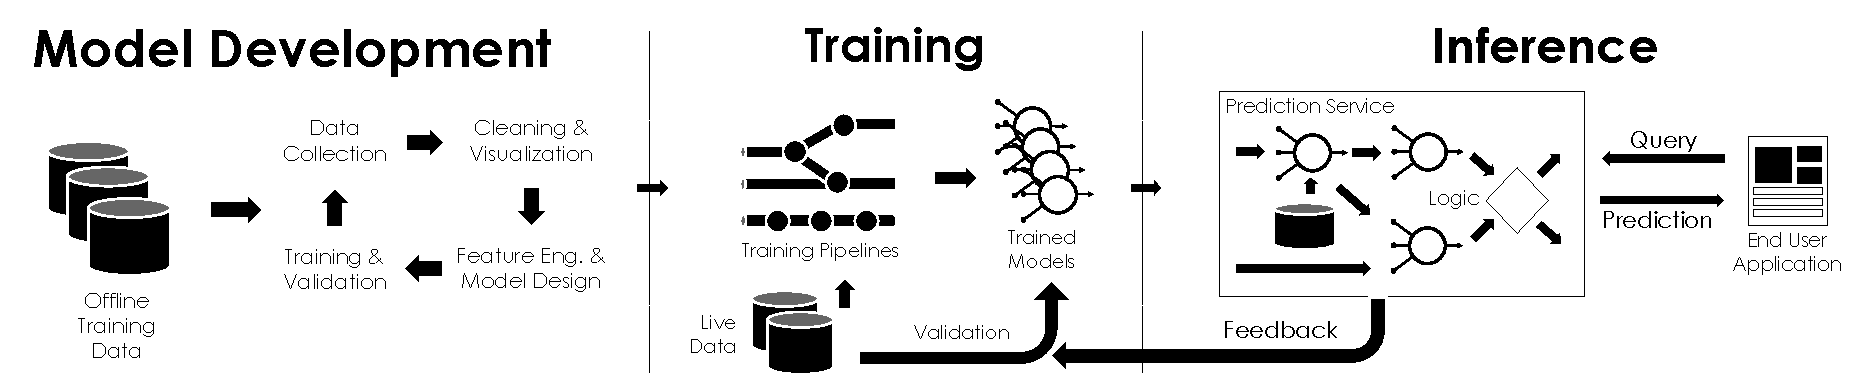
\includegraphics[width=\textwidth]{letters/pipeline.pdf}
\caption{\small \textbf{Machine Learning Life-cycle.} A simplified depiction of the key stages of a machine learning application.}
\label{fig:mllc}
\end{figure}


The machine learning life-cycle (Fig.~\ref{fig:mllc}) spans not only the model development, but also production training and inference.
Each stage demands different skills (e.g., neural network design, data management, and cluster management) and imposes different requirements on the underlying systems.
Yet there is an overwhelming need for unifying design principles and technologies to address pervasive problems including: feature management, data provenance, pipeline reproducibility, low-latency serving, and prediction monitoring just to name a few.


There has been substantial recent progress in systems to aid in managing the machine learning life-cycle.  
Large industrial projects like 
FB Learner Flow 
% \href{https://code.fb.com/core-data/introducing-fblearner-flow-facebook-s-ai-backbone/}{FB Learner Flow}
from Facebook, 
Michelangelo 
% \href{https://eng.uber.com/michelangelo/}{Michelangelo} 
from Uber, and 
TFX 
% \href{https://www.tensorflow.org/tfx/}{TFX} 
from Google have received a considerable of recent attention.  
In this issue we have solicited publications from several more recent industrial and academic projects.

The first paper, by a team at Amazon Research, provides an overview of several real-world use cases and then outlines the key conceptual, data management, and engineering challenges faced in production machine learning systems.
Rather than advocating a single system, this work describes some design principles that can inform potential solutions.


The second and third papers explores the challenges of model management and provenance across the machine learning life-cycle.
They motivate the need for systems to track models and their meta-data to improve reproducibility, collaboration, and governance. 
% expands upon the machine learning life-cycle 
% to include: data preparation, feature engineering, model training, deployment, and maintenance
% and explores the challenges of model 
The second paper introduces, ModelDB, an open-source system for model management and describe some of the functionality and design decisions. 
The third paper describes a related system, ProvDB, that uses a graph data model to capture and query fine-grained versioned lineage of data, scripts, and artifacts throughout the data analysis process.


The fourth paper, by a team at Databricks Inc., describes, MLFlow, a new open-source system to address the challenges of experimentation, reproducibility, and deployment. 
This work leverages containerization to capture the model development environment and a simple tracking API to enable experiment tracking.
The extensible model containerization enables model developers to more easily collaborate around modeling environments and then deploy model containers.


The last paper, by a team at Microsoft, focuses on inference and explores the challenges and opportunities of serving white-box prediction pipelines.  
In contrast to the containerization of pipelines in MLFlow, the Microsoft team leverage knowledge about the internal of the prediction pipeline to more efficient serve predictions. 



\end{document}




\end{letter}

\end{lettersection}

% put the name of your special issue below


\begin{opinionsection}
\begin{opinion}{A Wake-up Call: Managing Data in an Untrusted World}
{Divyakant Agrawal, Amr El Abbadi}{University of California, Santa Barbara}
\documentclass[11pt]{article}
%\usepackage[utf8]{inputenc}
\usepackage{url}

%\author{\\Department of Computer Science,
% University of California, Santa Barbara\\\textit{\{agrawal,}  \textit{amr\}@cs.ucsb.edu}}

\begin{document}
\title{A Wake-up Call: Managing Data in an Untrusted World}
\author{Divyakant Agrawal\qquad Amr El Abbadi\\
  University of California, Santa Barbara\\
  \textit{\{agrawal,}  \textit{amr\}@cs.ucsb.edu}}
%\maketitle
\vspace{1cm}

Once upon a time databases were structured, one size fitted all and they resided on machines that were trustworthy and even when they failed, they simply crashed.  This era has come and gone as eloquently stated by Stonebraker and Cetintemel~\cite{StonebrakerICDE2005}.  We now have key-value stores, graph databases, text databases, and a myriad of unstructured data repositories. The database community has wholeheartedly accepted the fact that the same information might come in different formats, modes and representations.  We also accept that data might not be "clean" and that data might need to be "cleaned" due to the diverse sources of information. However, we, as a database community still cling to our $20^{th}$ century belief that databases always reside on trustworthy, honest servers. Although the database community has always considered fault-tolerance as an integral building block of data management (remember "D" in ACID is for Durability), we still have trouble accepting the fact that not all failures are simply crash failures and might in fact involve malicious and non-trustworthy infrastructure. This notion has been challenged and abandoned by many other Computer Science communities, most notably the security and the distributed systems communities.  The rise of the cloud computing paradigm as well as the rapid popularity of blockchains demand a rethinking of our naïve, comfortable  beliefs in an ideal benign infrastructure.  In the cloud, clients store their sensitive data in remote servers owned and operated by cloud providers. The Security and Crypto Communities have made significant inroads to protect both data and access privacy from malicious untrusted storage providers using encryption and oblivious data stores.  The Distributed Systems and the Systems Communities have developed consensus protocols to ensure the fault-tolerant maintenance of data residing on untrusted, malicious infrastructure.  However, these solutions face significant scalability and performance challenges when incorporated in large scale data repositories. Novel database designs need to directly address the natural tension between performance, fault-tolerance and trustworthiness.  This is a perfect setting for the database community to lead and guide.  

In this opinion article, we will illustrate an interesting atomicity problem in the context of exchanging cryptocurrencies using permissionless blockchains. We also illustrate that transaction management can learn from the blockchain approach when attempting to restricted untrusted behaviour from the underlying infrastructure.  We hope this will illustrate some of the challanges that need to be addressed in malicious, untrusted settings, as well as connections with standard database problems like commitment, replication and transaction management in general. 

Bitcoin~\cite{nakamoto2008bitcoin} took the world by surprise over a decade ago by introducing a novel cryptocurrency, which supports the execution of transactions, albeit relatively simple transfers.  As with any data management system, bitcoin needed to address the challenge of durability.  Its approach, rather than using a trusted persistence storage device to store the current state, e.g., a disk, relies on global replication of a distributed data structure called a {\em blockchain}.  A blockchain is basically a linked list of blocks, each of them containing a set of transactions.  The blockchain is replicated on a potentially unknown number of {\em untrusted} servers.
Two of the main challenges that bitcoin needed to address are (1) the unknown number of participants and (2) the untrusted nature of the participants.  The former challenge basically manifests itself when consensus is needed to add a new block to the blockchain.  This is resolved by avoiding communication to achieve consensus, as is typical in Byzantine Agreement protocols, and replacing it with computation, namely the well-known {\em Proof of Work} mining puzzle operation.  The latter challenge is addressed using many different cryptographic techniques, including digital signatures, hash pointers, etc.  Currently, it seems that database vendors have adopted blockchains, with their untrusted infrastructure, but only in contexts where the number of untrusted participants is known {\em a priori}.  This problem is suitable for supply-chain, financial and healthcare applications. In blockchain terminology, this is referred to as {\em permissioned blockchains}.  Over the past few years different permissioned blockchain systems have been developed in both
industry and academia.
Some known industrial permissioned blockchain systems include Hyperledger Fabric \cite{androulaki2018hyperledger} which was introduced by IBM and is widely used in supply chain management,
Quorum \cite{morgan2016quorum} by JPMorgan which supports financial applications, and
Libra \cite{libra2019libra} is a digital currency by Facebook.
Similarly, in academia, Fast Fabric \cite{fastfabric2019}, ParBlockchain \cite{amiri2019parblockchain},
ResilientDB \cite{gupta2020resilientdb}, Caper \cite{amiri2019caper}, AHL \cite{dang2018towards}, etc. have been proposed. This is a good step, and demonstrates our willingness to address the challenges of untrusted as well as unreliable infrastructures.  However, we believe database researchers have a lot more to offer.  These efforts go in both directions, i.e., to extend support for untrusted infrastructures in diverse data management contexts, as well as exploiting data management techniques in diverse novel and non-traditional contexts, as for example in permissionless blockchains.


Bitcoin and other cryptocurrencies are {\em permissionless} blockchains.
In a permissionless blockchain, the network is public, and anyone can participate without a specific identity.
The recent adoption of blockchain technologies and open 
permissionless networks has demonstrated user needs to exchange assets
and especially without depending on centralized 
intermediaries such as banks or exchanges. 
This problem requires infrastructure enablers and protocols that allow users to 
{\em atomically} exchange assests without giving up trust-free decentralization,
the main reasons behind using  permissionless blockchain. We motivate the problem
of atomic cross-chain transactions and discuss
the current available solutions and their limitations through the following example.  

Suppose Alice owns X bitcoins and she wants to exchange them for Y 
ethers. Luckily, Bob owns ether and he is willing to exchange his Y ethers for X bitcoins. 
In this example, Alice and Bob want 
to atomically exchange assets that reside in different blockchains. In addition,
both Alice and Bob \textit{do not trust} each other and in many scenarios, 
they might not be co-located to do this atomic exchange in person.
Current infrastructures
do not support these direct peer-to-peer transactions. 
Instead, both Alice and Bob need to \textit{independently} exchange their 
assets through a trusted centralized exchange, Trent 
(e.g., Coinbase~\cite{coinbase} and Robinhood~\cite{robinhood}) either through
fiat currency or directly.  Using fiat, both Alice
and Bob first exchange their assets with Trent for a fiat currency (e.g., USD) and 
then use the earned fiat currency to buy the other assets also from Trent or from 
another trusted exchange. Alternatively, some exchanges (e.g., Coinbase) allow their 
customers to directly exchange assets (ether for bitcoin or bitcoin for ether) 
without going through fiat currencies.

A two-party cross-chain commitment protocol was originally proposed by 
Nolan~\cite{atomicNolan} and generalized by 
Herlihy~\cite{herlihy2018atomic} to process multi-party cross-chain transactions, or swaps.
Both Nolan's protocol and its generalization by Herlihy use smart contracts, hashlocks,
and timelocks to execute cross-chain transactions. A {\em smart contract} is a self executing
contract (or a program) that is executed in a blockchain 
once all the terms of the contract are satisfied. A {\em hashlock} is 
a cryptographic one-way hash function $h = H(s)$ that locks
assets in a smart contract until a hash secret $s$ is provided. A {\em timelock} is a time 
bounded lock that triggers the execution of a smart contract function
after a pre-specified time period. 
%It is interesting to note how many of these basic tools are quite familiar to database practitioners.
These proposals solve the cross-chain commitment problem and ensure that untrusted participants comply and do not try to misuse the system.
However, an expired timelock could lead to a violation of the all-or-nothing
atomicity property. An honest participant who fails to react in time due to a crash failure, network delays or even a denial of service attack 
might end up losing their assets. Although a crashed participant
is the only participant who ends up worse off, current proposals are
unsuitable for atomic cross-chain transactions in asynchronous 
environments where crash failures and network delays are the norm. 
This is a problem familiar to the database community since its inception, namely the {\em atomic commitment problem}.  In~\cite{zakhary2020atomic}, we present a decentralized all-or-nothing \textit{atomic} cross-chain commitment protocol.  Events for redeeming and refunding smart contracts to exchange assets are 
modeled as conflicting events. An open permissionless network of witnesses is 
used to guarantee that conflicting events could never simultaneously occur 
and either all smart contracts in an atomic cross-chain transaction
are redeemed or all of them are refunded.  A similar protocol was also concurrently proposed by Herlihy et al.~\cite{Herlihy2020VLDB}, which addresses the same atomicity challenge, but in the context of {\em cross chain deals}, where a {\em deal} is a weaker notion of an atomic transaction.

Now, we briefly come back to traditional databases and large scale data fault-tolerant transaction management but on untrusted infrastructures.  As increasing amounts of data are currently being stored and managed on third-party servers, there is emerging demand for a suite of protocols to manage data on untrusted infrastructures. In Fides~\cite{maiyya2020fides}, we introduce a novel atomic commitment protocol, TFCommit, that executes transactions on data stored across multiple untrusted servers. This novel atomic commitment protocol executes transactions in an untrusted environment without the need for expensive Byzantine replication. One main obstacle for the adoption of Byzantine Agreement protocols are the various impossibility results, that require {\em a priori} knowledge of the maximum possible number of failures in the system (e.g., one third in case of malicious failures).  From a practical point of view, this might be difficult to ascertain.  We propose using TFCommit in an {\em auditable} data management system, Fides, residing completely on untrustworthy infrastructures. As an auditable system, Fides guarantees the detection of potentially malicious failures occurring on untrusted servers using blockchain inspired tamper-resistant logs with the support of cryptographic techniques. As a result, Fides is scalable and does not require any {\em a priori} known bounds on the number of malicious faults when executing transactions on untrusted infrastructure.  If malicious behaviour occurs, it is recorded and can be detected by an external auditor.  Just the threat of investigation should usually deter improper behaviour.

In conclusion, we encourage researchers to explore a relatively new and uncharted domain for the database community.  Many techniques have indeed been developed by the security, cryptography and distributed systems communities.  However, these solutions are often too expensive to use in the practical scalable settings data management systems encounter on a daily basis. 
In fact, we view this as a two way exchange of ideas and innovations.  Over four decades of fault-tolerant data management innovations can be beneficial and can have significant impact in solving many of the practical large scale problems that need to be addressed in untrusted infrastructures.   On the other hand, many of the techniques developed to restrict malicious behaviour using cryptographic and distributed computing approaches can facilitate the development of fault-tolerant database management systems in untrused infrastructures, which are becoming more prevalent and commonplace for storing data.
\section*{Acknowledgement}

This work is partially funded by NSF grants CNS-1703560 and CNS-1815733.

\begin{thebibliography}{10}

\bibitem{coinbase}
Coinbase.
\newblock \url{https://coinbase.com}, 2018.

\bibitem{robinhood}
Robinhood.
\newblock \url{https://robinhood.com/}, 2018.

\bibitem{amiri2019caper}
Mohammad~Javad Amiri, Divyakant Agrawal, and Amr~El Abbadi.
\newblock Caper: a cross-application permissioned blockchain.
\newblock {\em Proceedings of the VLDB Endowment}, 12(11):1385--1398, 2019.

\bibitem{amiri2019parblockchain}
Mohammad~Javad Amiri, Divyakant Agrawal, and Amr~El Abbadi.
\newblock Parblockchain: Leveraging transaction parallelism in permissioned
  blockchain systems.
\newblock In {\em 39th International Conference on Distributed Computing
  Systems (ICDCS)}, pages 1337--1347. IEEE, 2019.

\bibitem{androulaki2018hyperledger}
Elli Androulaki, Artem Barger, Vita Bortnikov, Christian Cachin, et~al.
\newblock Hyperledger fabric: a distributed operating system for permissioned
  blockchains.
\newblock In {\em EuroSys Conference}, page~30. ACM, 2018.

\bibitem{morgan2016quorum}
JP~Morgan Chase.
\newblock Quorum white paper, 2016.

\bibitem{dang2018towards}
Hung Dang, Tien Tuan~Anh Dinh, Dumitrel Loghin, Ee-Chien Chang, Qian Lin, and
  Beng~Chin Ooi.
\newblock Towards scaling blockchain systems via sharding.
\newblock In {\em Proceedings of the 2019 ACM SIGMOD International Conference
  on Management of Data}. ACM, 2019.

\bibitem{fastfabric2019}
Christian Gorenflo, Stephen Lee, Lukasz Golab, and S.~Keshav.
\newblock Fastfabric: Scaling hyperledger fabric to 20,000 transactions per
  second.
\newblock {\em arXiv preprint arXiv:1901.00910}, 2019.

\bibitem{gupta2020resilientdb}
Suyash Gupta, Sajjad Rahnama, Jelle Hellings, and Mohammad Sadoghi.
\newblock Resilientdb: Global scale resilient blockchain fabric.
\newblock {\em arXiv preprint arXiv:2002.00160}, 2020.

\bibitem{herlihy2018atomic}
Maurice Herlihy.
\newblock Atomic cross-chain swaps.
\newblock In {\em ACM Symposium on Principles of Distributed Computing (PODC)},
  pages 245--254. ACM, 2018.

\bibitem{Herlihy2020VLDB}
Maurice Herlihy, Liuba Shrira, and Barbara Liskov.
\newblock Cross-chain deals and adversarial commerce.
\newblock {\em Proc. {VLDB} Endow.}, 13(2):100--113, 2019.

\bibitem{maiyya2020fides}
Sujaya Maiyya, Danny Hyun~Bum Cho, Divyakant Agrawal, and Amr~El Abbadi.
\newblock Fides: Managing data on untrusted infrastructure.
\newblock {\em arXiv preprint arXiv:2001.06933}, 2020.

\bibitem{libra2019libra}
Libra~Association Members.
\newblock An introduction to libra.
\newblock {\em https://libra.org/en-US/white-paper/}, 2020.

\bibitem{nakamoto2008bitcoin}
Satoshi Nakamoto.
\newblock Bitcoin: A peer-to-peer electronic cash system.
\newblock 2008.

\bibitem{atomicNolan}
Tier Nolan.
\newblock Alt chains and atomic transfers.
\newblock
  \url{https://bitcointalk.org/index.php?topic=193281.msg2224949#msg2224949},
  2013.

\bibitem{StonebrakerICDE2005}
Michael Stonebraker and Ugur {\c{C}}etintemel.
\newblock "one size fits all": An idea whose time has come and gone (abstract).
\newblock In Karl Aberer, Michael~J. Franklin, and Shojiro Nishio, editors,
  {\em Proceedings of the 21st International Conference on Data Engineering,
  {ICDE} 2005, 5-8 April 2005, Tokyo, Japan}, pages 2--11. {IEEE} Computer
  Society, 2005.

\bibitem{zakhary2020atomic}
Victor Zakhary, Divyakant Agrawal, and Amr El~Abbadi.
\newblock Atomic commitment across blockchains.
\newblock {\em Proceedings of the VLDB Endowment}, 13:1, 2020.

\end{thebibliography}
\end{document}

\end{opinion}
\begin{opinion}{The Battle for Data Science}
{Jeffrey D. Ullman}{Stanford University}
\documentclass[11pt]{article} 
\usepackage{deauthor,times,graphicx}%,hyperref} 

\begin{document}
\title{The Battle for Data Science}
\author{Jeffrey D. Ullman\\Stanford University, Dept.\ of Computer Science\\ullman@gmail.com}

%\maketitle

\section{Introduction}

Through the years, the database community has periodically looked at developments in technology and engaged in hand-wringing over the idea that we are becoming irrelevant.  The cry ``have we missed the boat~-- again'' is common; e.g., here is a panel I served on several years ago \cite{boat}.
My goal in this essay is to argue that the database field and the techniques that have come from this research are still essential for ``data science,'' that is, for the exploitation of data to solve problems of importance in application fields~-- science, commerce, medicine and such.  I believe, as I assume most readers of this article believe, that the field of database systems has always had at its core the study of how to deal with the largest amounts of data possible at the time, whether that be megabytes of corporate payroll data, terabytes of genomic information, or petabytes of satellite output.  Thus whatever study of data is necessary at the time~-- that's our job.

To advance this argument, I want to look at three issues:

\begin{enumerate}

\item
Is the field of statistics really the essential ingredient in data science?

\item
Is machine learning really what data science is all about?

\item
Is data science a danger to decent societal norms?

\end{enumerate}
Hint: my answer to all three is ``no.''  I'll try to address each of these in turn.

\section{The Battle Line: Venn Diagrams for Data Science}

Several years ago, I was invited to a panel of the National Research Council called the ``Data-Science-Education Roundtable.''  The output of this group can be seen at \cite{dsr}.  It was organized not by the computer-science wing of the NRC but the statistics branch.  The participants were roughly equally divided between  statisticians and computer scientists, plus a few from other disciplines.  Part of my experience was seeing how statisticians thought about the world of data and its application.  The most obvious point was that the field of statistics views data science as its own.

To be fair, let's be clear at the outset that I have great respect for statisticians and the work they do.
Statistics has become increasingly important to the modern study of data, including, but not limited to machine learning.
Many statisticians are starting to focus on computation and data analysis in the same way as we do in the database community or in
computer science more generally.  Just to offer one small example, one of my favorite techniques is locality-sensitive hashing, which is an
idea that came squarely out of the database community \cite{lsh}.   Yet one of my colleagues in the Statistics Department at Stanford, Art Owen,
showed me something \cite{owen} about a key step, minhashing \cite{minhash}, that speeds up the process by a very large factor -- something we should have been able to figure out years ago, but didn't.

However, my experience in the roundtable also gave me the sense that there is an effort on the part of some in the statistics community to define statistics as the central component of data science.  I, in contrast, would see the algorithms and techniques for processing large-scale data efficiently as the center of data science.  There is a general sense that data science is a discipline that combines the knowledge of several fields, and I agreed completely.  But what are those fields, and how do they interact?  The question is considered so important that competing communities have published Venn diagrams to justify their own centrality in data science.  There was a recent article \cite{venn} summarizing and commenting upon  a number of these diagrams.  Or if you really want to see the full spectrum of viewpoints expressed as venn diagrams, issue the search query [wikipedia data science venn diagrams].

\subsection{The Conway Diagram}

It appears that statisticians all use a particular diagram, due to Drew Conway.  This diagram shows three sets intersecting: ``hacking skills,'' ``math and statistics,'' and ``substantive expertise.''  At the roundtable, this diagram was shown several times to illustrate the importance of statistics, and I have seen statisticians in several other contexts showing the same diagram to explain the importance of their field to data science.  I reproduce the diagram in Fig.~\ref{drew-diagram-fig}, but I have added my own edits and comments to explain what is misleading about the diagram.

\begin{figure}[h]
\centerline{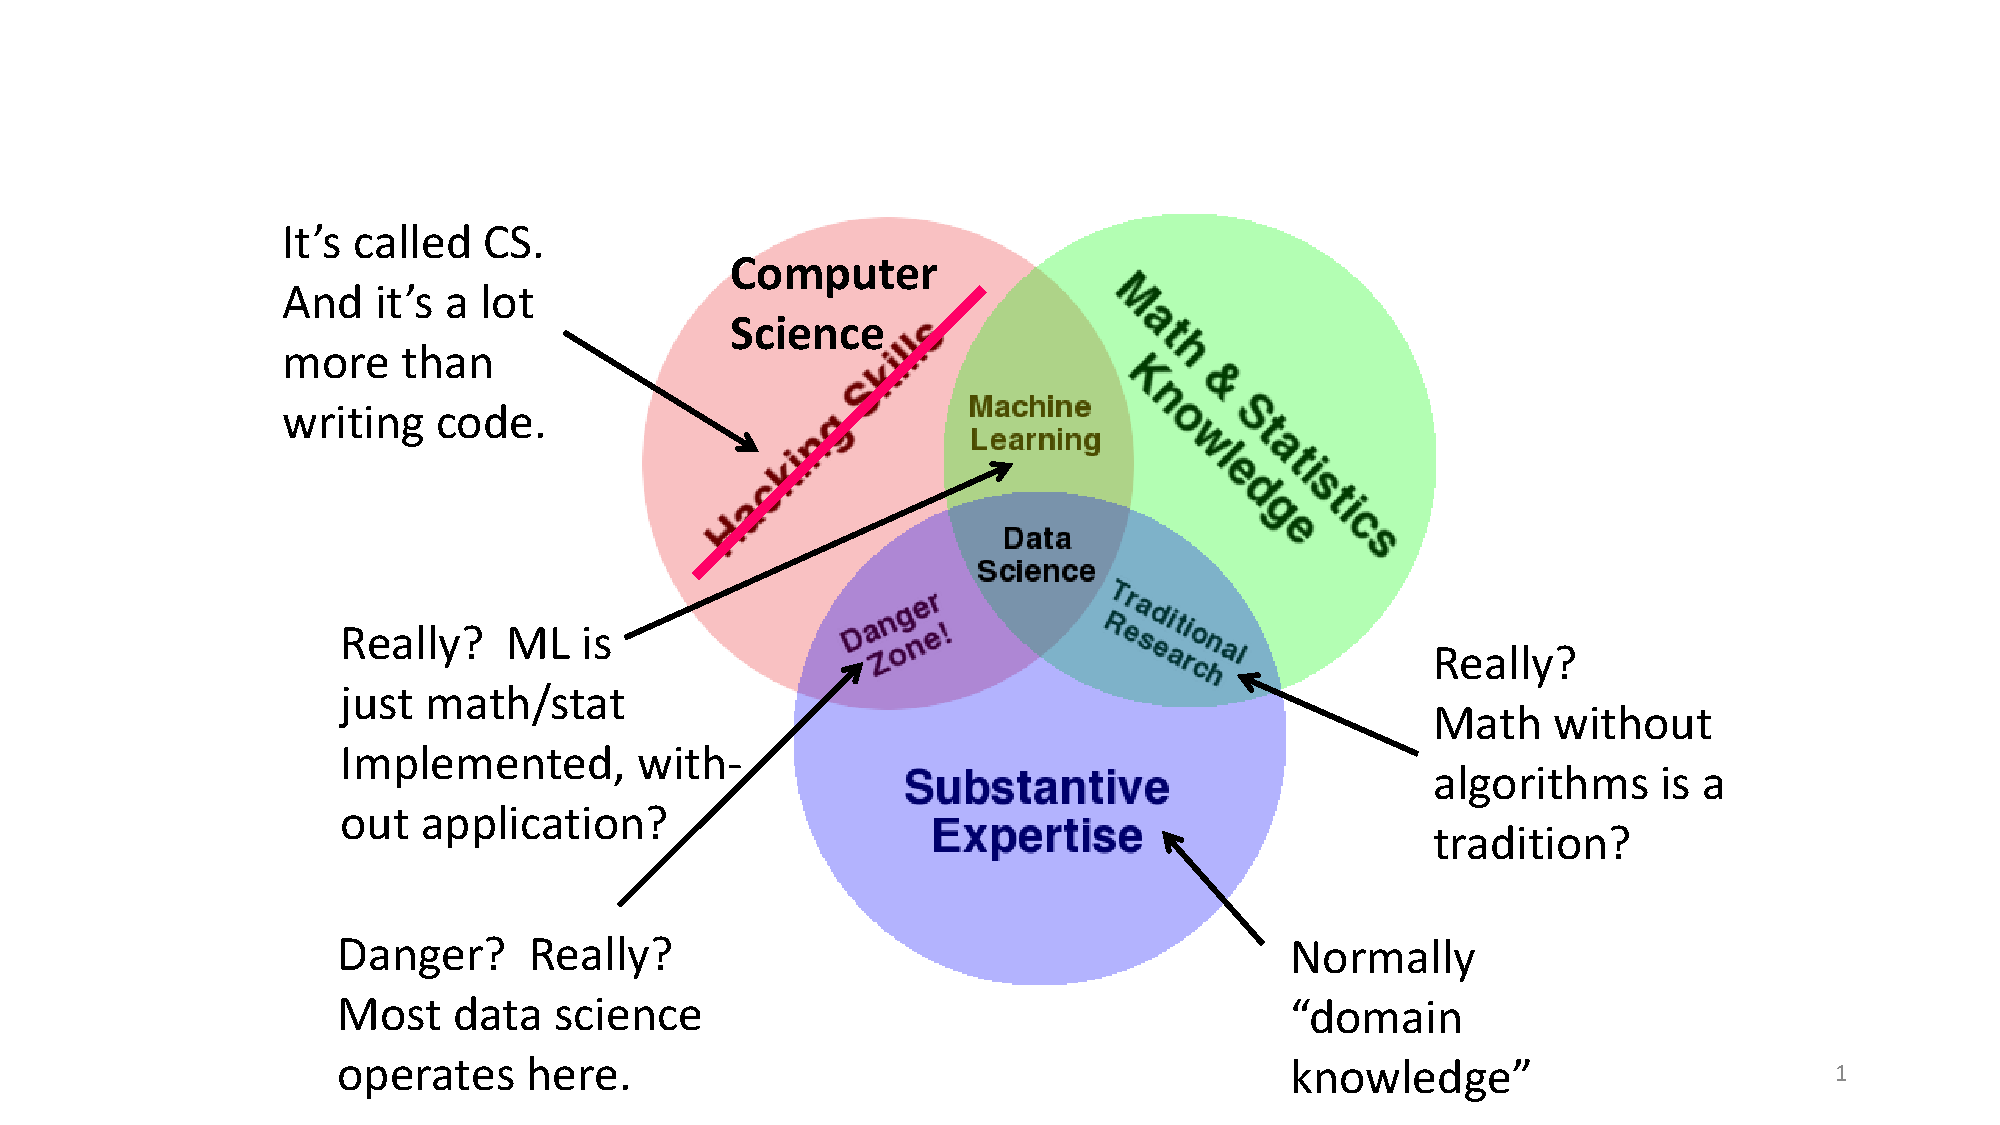
\includegraphics[width=0.8\textwidth]{letters/drew-diagram.pdf}}
\caption{The Conway Venn diagram for data science}
\label{drew-diagram-fig}
\end{figure}

In fact, almost every region of the diagram is misleading in some way.

\begin{enumerate}

\item
First, a small matter: what is referred to as ``substantive expertise'' is generally called ``domain knowledge'' or something similar.

\item
The most egregious impropriety is referring to computer science as ``hacking skills.''  Computer science brings far more to data science than the ability to write code.  We offer algorithms, models, and frameworks, for solving problems of all sorts.  All of that is essential in dealing with data.

\item
``Traditional research'' is shown in the diagram as math/stat intersected with applications.  In other words, in this form of research, one thinks about the application, but does not write any code, and therefore there is nothing that affects the real world.  I don't know whose tradition that is, but I am glad to say it is not the tradition of the database community.

\item
Machine learning has an odd place in this diagram.  It is described as ``hacking'' plus math/stat.  The implication is that machine learning has nothing to do with applications.  In practice, it has everything to do with applications, which is why today the algorithms from machine learning are taken so seriously, not only in the database community, but all across computer science.

\item
And then there is what Conway calls the ``danger zone''~-- writing code to solve problems in application areas without the wise guidance of a statistician.  Well almost all of data science is like that.  For just one example, Google and other mail services are pretty good at detecting phishing emails.  How good?  We really don't know, and even if we could do a statistical analysis today, it would not be valid tomorrow, as the threats change.  The real danger would be refusing to do the best we could, and letting some poor soul send their life savings to some scam artist.

\end{enumerate}

\subsection{My Venn Diagram}

I too offered a Venn diagram (Fig. \ref{myvenn-fig}) that I believe better represents the relationships between the fields.  There is computer science and the various domain sciences, and somewhere in the intersection of these is data science.  Machine learning is a branch of computer science~-- a very important subset these days.  Some of machine learning is used for data science, although there are other uses of machine learning that are more internal to computing.  Many of these applications are considered ``artificial intelligence'' these days, e.g., driverless cars or intrusion detection.  Finally, I see both math and statistics as very important tools for all of computer science, and the small bubbles in my diagram do not do justice to their importance.  However, I drew them as shown to emphasize that they do not really impact domain sciences directly.  but rather they do so through the software that is developed, often with their important aid.

\begin{figure}[h]
\centerline{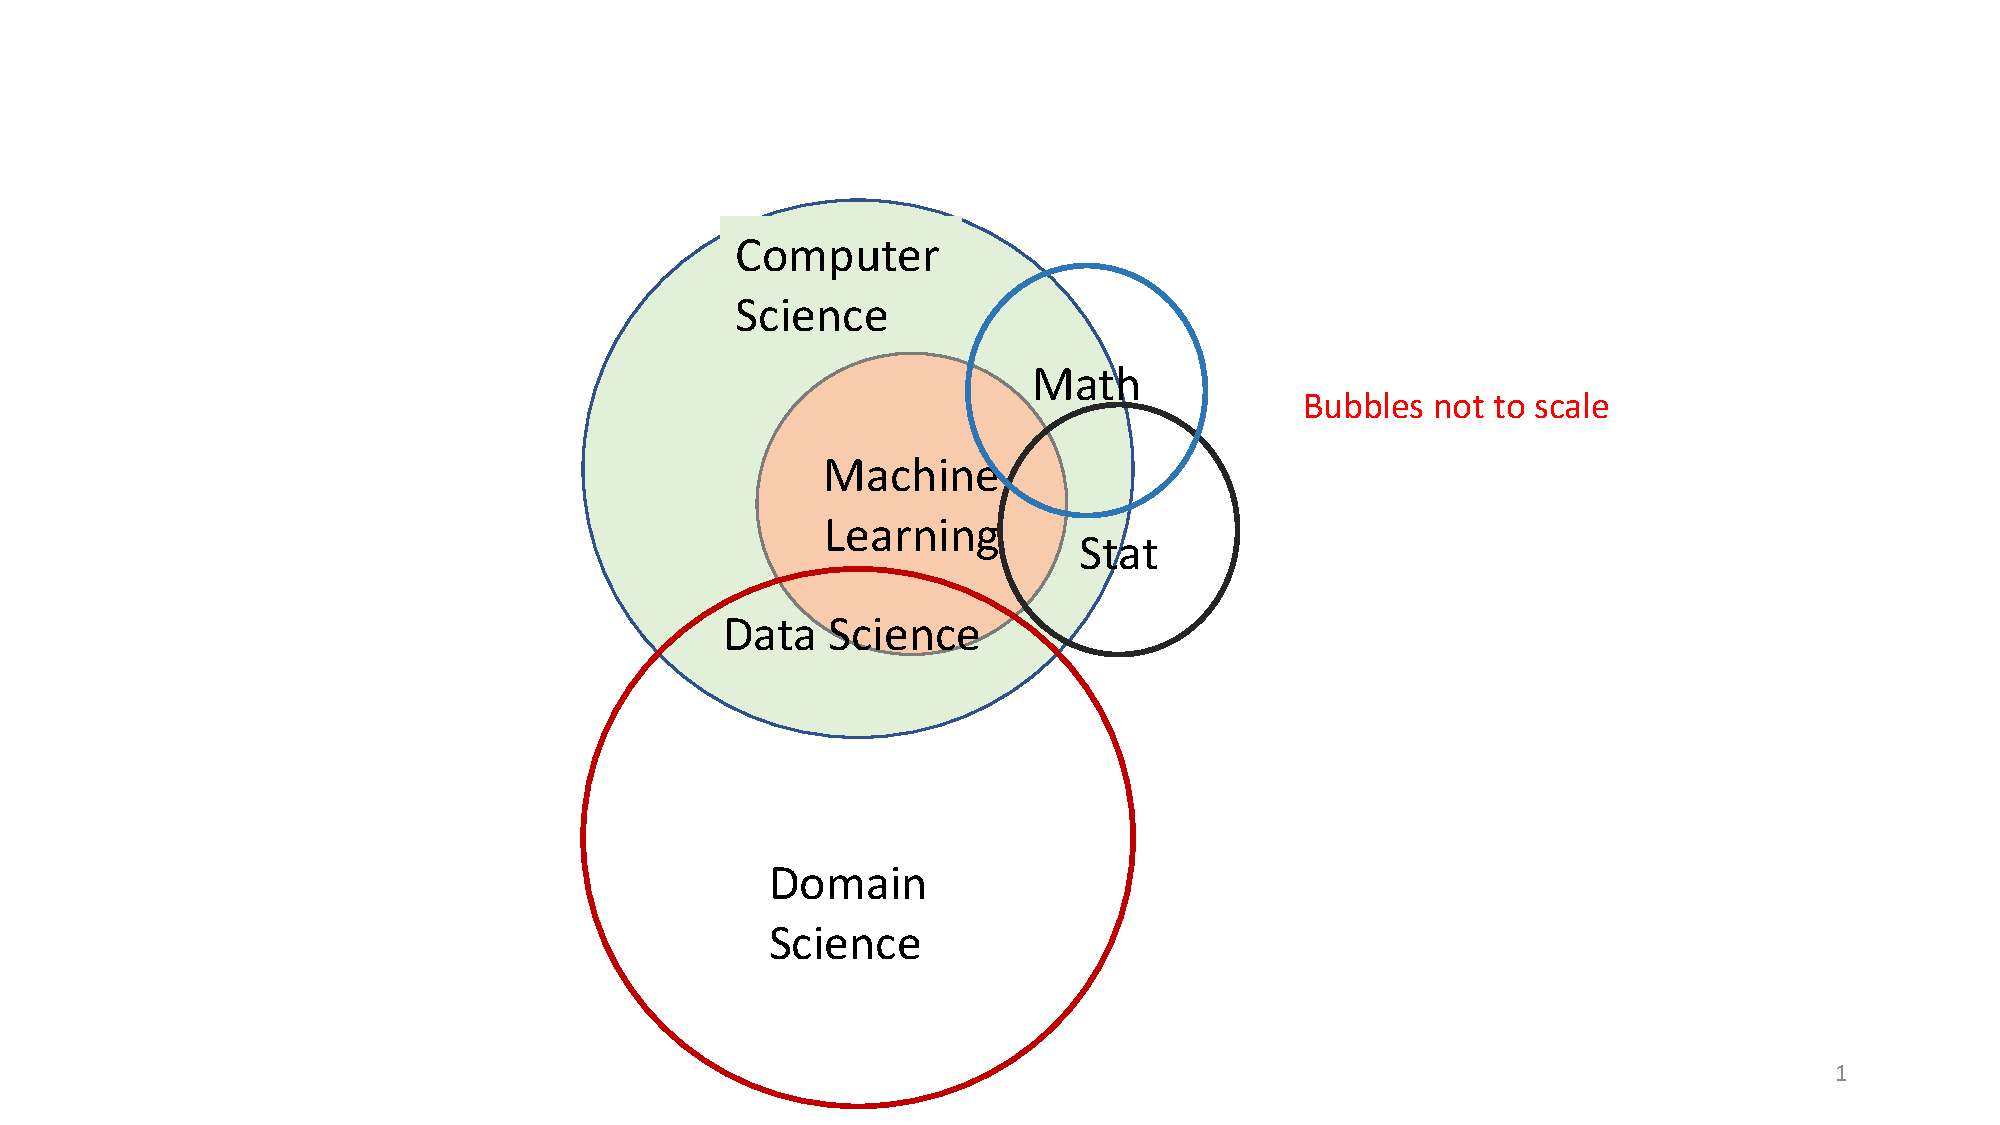
\includegraphics[width=0.8\textwidth]{letters/myvenn.pdf}}
\caption{A personal view of the relationship between computer science, machine learning, and statistics}
\label{myvenn-fig}
\end{figure}

\subsection{The Big Difference: Database and Statistics Value Systems}

Perhaps the most contentious implication of my diagram is that math/stat does not address domain applications directly.  After all, the Conway diagram talks about ``traditional research'' as doing just that.  But while there may be interaction between applications and math/stat that bypasses computing, I think it is rare that the interaction results in any benefit to the application.

To illustrate the distinction, look at the report of the fourth meeting of the data-science education roundtable \cite{datafest}.  One part of the discussion centered on the ``hackathon'' run by the American Statistical Association, called ``Datafest.''  Superficially, this event is just like the sort of hackathon we see run for computer-science students.  The competing teams are given a large dataset, drawn from some application area.  But there is a big difference in how the competition is evaluated.  Competitors are not expected to solve someone's problem, and are not evaluated on the quality of their solution.  Rather, ``awards were given for best data visualization, best use of external data, and best insight.''  In other words, you win a statistical hackathon by doing something of interest to statisticians, not by solving someone else's problem.  I hope the reader appreciates the opposite approach, where the goal is to serve, not to amuse oneself.  That approach, for example, is what drives the computer-science-oriented Kaggle competitions \cite{kaggle}.

\section{Database Systems and Machine Learning}

Now, let us turn to how the rise of machine learning has impacted the use of data.  There is no question that machine learning has had enormous impact on our ability to use data to solve problems.  Many of the most impressive recent achievements have been applications of algorithms in the machine-learning class.  However, I do not believe that machine learning is a complete replacement for the algorithms that have been developed in the database community.  I wish the reader to consider three issues:

\begin{enumerate}

\item
There are many problems involving ``big data'' that are not really machine-learning problems.

\item
Not everything that machine learning claims as its own really comes from there.

\item
Many machine-learning methods produce mysterious models that do not support explanation or justification.

\end{enumerate}

\subsection{Machine Learning Is Not All of Data Science}

I believe a fair definition of machine learning is algorithms that use data to create a model of something, from which answers can be derived.  For example, machine learning can be used to build a model of spam emails, so that a given email can be fed to the model and reliably found to be spam or not spam (``ham'').  But not every useful solution can be expressed as a model.  For example, we earlier mentioned locality-sensitive hashing (LSH) as an important technique from the database community for dealing with data.  LSH is a body of techniques (see, e.g., Chapter 3 of \cite{mmds}) for finding similar items in a dataset without having to look at all pairs.  You don't need for the dataset to be very large before looking at all pairs is prohibitive; even a million items in your set implies half a trillion pairs that would need to be looked at.  So when applicable, LSH can be a very powerful tool.  But there is no model involved.  It is not an instance of machine learning.

\subsection{Machine-Learning Advocates Sometimes Claim Too Much}

I have heard of clustering, for example, defined as a branch of machine learning, even though clustering has been studied from well before there was such a thing as machine learning.  Gradient descent is another example of something that predates machine learning, yet somehow is popularly regarded as a machine-learning topic.  Another important example concerns {\em association rules}.  This idea was pioneered in 1993--4 by Rakesh Agrawal and his friends \cite{ais} \cite{as} and predates almost all of machine learning.   I even recall talking to a machine-learning advocate and offering LSH as an example of a big-data algorithm that had nothing to do with machine learning.  His response was that LSH ``must be machine learning, because it is a really good idea.''

\subsection{Explainability}

Often, a machine-learning algorithm draws correct conclusions that cannot be explained except by showing the model.  And that model is often so complex that it means nothing to the average user.  Sometimes, no one cares; the important thing is that the model, say, gives the correct diagnosis, even if its reasoning is hidden in the processing of a megapixel image.  On the other hand, sometimes, we have a right to an explanation.  For example, if your insurance company raises your rates because some model of automobile accidents has decided you are more likely to have an accident than the previous model showed, it seems proper that you at least be told why this is happening to you.  In Europe, the GDPR laws \cite{gdpr} guarantee you that right.

But non-machine-learning approaches are often more explainable than machine-learning models.  To see the difference, let us reconsider the matter of association rules as a way to identify spam emails.  One would produce a set of ``rules,'' which in this case would be sets of words, whose presence in an email indicates it is spam.  You might think of these rules as a model of spam, which is probably why machine-learning advocates view the method as their own.  But in fact, the algorithms used to find association rules do not ``learn'' a model from the data.  They simply count the number of spam emails that contain certain sets of words, and if that count is high enough, they declare a rule that emails containing that set of words is spam.  For instance, we might expect that one rule would say that emails containing the set $\{${\tt Nigerian}, {\tt prince}$\}$ are spam.  In contrast, even the simplest machine-learning technique, such as learning a (positive or negative) weight on each possible word, and declaring spam if the sum of the weights exceeds a threshold, will be more accurate than a solution based on association rules.

However, the association-rule approach is explainable, while the machine-learning model is not.  If I really {\em am} a Nigerian prince, and all my emails are sent to spam, at least I can understand why.  On the other hand, if you have ever asked gmail why it declared something to be spam, its usual answer is something like ``it looked like other emails that were spam.''  That is, whatever model we are using today said it was spam, and that's all we can tell you.\footnote{Interestingly, I was the victim in way similar to that of the hypothetical Nigerian prince.  A dean asked me for a letter concerning a candidate for promotion, which I sent.  He claimed the email never arrived, so I sent it again.  It never arrived.  Eventually, he discovered that the mail system at his university had a rule that said anything from my email address was to be discarded immediately.  I suspect someone at some time engaged in a denial-of-service attack using my faked email address.  At least we were able to understand the problem and get it fixed quickly.}

\section{Attacks on the Use of Data}

It is common to blame data for the ills of society.  However, the fault rarely lies in the idea of using data to address a social issue.  Rather, the source of error is more likely to come from:

\begin{enumerate}

\item
People intentionally or unintentionally misusing the data, or

\item
Problems in the reality that the data faithfully reflects.

\end{enumerate}

\subsection{Misuse of Data}

At the Data-Science-Education Roundtable, there was a discussion in the fifth session on data ethics, which you may find in \cite{ethics}.  One common problem discussed was the use of ``false proxies.''  For an example given there, a city wants to deploy its police to the areas where crime occurs.  What they have is data on where arrests occur, so they send their police there, and lo and behold, they arrest more from those areas.  But arrests do not reflect solely the occurrence of crime; they also reflect the presence of police to make the arrests.  So a possible error is perpetuated by the data.  That is, if for bad reasons, police had been sent to certain areas preferentially in the past, the data will truly reflect that there are more arrests in those areas.  Perhaps, just as much crime occurs elsewhere, but the arrest rate is lower in places where the police presence is low.

Another common example of where data can perpetuate bias concerns a hypothetical company that has always discriminated against women when promotions are handed out.  They want to build an AI system using machine learning, to process resumes and identify those with characteristics similar to those of their successful employees.  But the data shows that being female is an indication that the candidate will not be successful, so the machine-learning algorithm learns from the data to reject applications from females.   The data again perpetuates an existing bias.  But the data didn't create the bias; people did.

\subsection{Data Reflecting a World We Don't Like}

A less reasonable charge against the use of data is that the resulting systems reflect something about society that the speaker opposes.  A clear example of this sort of false reasoning concerns Word2Vec \cite{word2vec}, a system developed at Google several years ago (since popularly superseded by an alternative system called BERT \cite{bert}) that embeds words in a high-dimensional vector space, in such a way that words with similar meaning have vectors that are close.  The intuitive idea is to look at the words that typically surround the word $w$ in question.  The vector for $w$ then is a weighed combination of directions associated with its surrounding words.  For example, we would expect {\tt Coke} and {\tt Pepsi} to have similar vectors, because people talk about them in much the same way.

The problem arose when it was observed that certain vector equations were approximately followed.  For example, as vectors,

\begin{center}
{\tt London} $-$ {\tt England} + {\tt France} = {\tt Paris}
\end{center}
That is, London and Paris, being the capitals and largest cities of their respective countries, have around them many words reflecting that status.  However, we would expect London to have more words that are associated with England surrounding it, so take them away and substitute words associated with France.

No one was disturbed by that observation, but other equations raised some hackles.  For instance, \cite{buono} called out the equation

\begin{center}
{\tt doctor} $-$ {\tt man} + {\tt woman} = {\tt nurse}
\end{center}
A similar objection to another such equation is discussed in \cite{boluk}.  However, if you look at this equation, it is asking ``find me a profession like doctor, but with more females.  About 50\% of doctors are women, but close to 90\% of nurses are women.  We expect that words surrounding {\tt doctor} and {\tt nurse} would be similar, but the latter will more often be found near words like {\tt she}.  So the equation makes sense.  What these negative articles are really objecting to is a society where women are more likely to be channeled into nursing.  I agree, and probably in the not-too-distant future, that will not be the case.  But my point is: don't blame the data.  Systems like Word2Vec or BERT, when trained on a large corpus like Wikipedia, will reflect language as used by a broad segment of the public, and that usage will in turn reflect what is generally thought to be true, regardless of whether we like that truth or not.

\section{The Last Word}

I hope the reader will take away the following thoughts:

\begin{itemize}

\item
Data and its management is still the essence of data science.

\item
While machine learning is very important, it is far from the only tool or idea needed for effective data science.

\item
Although there have been misuses of data, we should not blame data if it reflects the world as it is, rather than as we would like it to be.

\end{itemize}

\vspace{-.1cm}
\bibliographystyle{ACM-Reference-Format}
\begin{thebibliography}{10}
\begin{small}
\itemsep=-.5pt

\bibitem{ais}
R. Agrawal, T. Imielinski, and A. Swami,
``Mining associations between sets of items in massive databases,''
{\em Proc.\ ACM SIGMOD Intl.\ Conf.\ on Management of Data},
pp.~207--216, 1993.

\bibitem{as}
R. Agrawal and R. Srikant,
``Fast algorithms for mining association rules,''
{\em Intl.\ Conf.\ on Very Large Databases}, pp.~487--499, 1994.

\bibitem{boluk}
T. Bolukbasi, K.-W. Chang, J. Zou, V. Saligrama, and A. Kalai,
``Man is to computer programmer as woman is to homemaker? Debiasing word embeddings,''
{\em 30th Conference on Neural Information Processing Systems}, Barcelona, 2016.

\bibitem{minhash}
A.Z. Broder, M. Charikar, A.M. Frieze, and M. Mitzenmacher,
``Min-wise independent permutations,''
{\em ACM Symposium on Theory of Computing}, pp.~327--336, 1998.

\bibitem{buono}
T. Buonocore, ``Man is to doctor as woman is to nurse: the gender bias of word embeddings,'' https://towardsdatascience.com/gender-bias-word-embeddings-76d9806a0e17

\bibitem{bert}
J. Devlin, M.-W. Chang, K. Lee, and K. Toutanova,
``BERT: Pre-training of deep bidirectional transformers for language understanding,''
arXiv:1810.04805, 2018.

\bibitem{lsh}
A. Gionis, P. Indyk, and R. Motwani,
``Similarity search in high dimensions via hashing,''
{\em Proc.\ Intl.\ Conf.\ on Very Large Databases}, pp.~518--529, 1999.

\bibitem{boat}
B. Howe, M.J. Franklin, L.M. Haas, T. Kraska, and J.D. Ullman:
``Data science education: we're missing the boat, again,'' {\em ICDE}, pp.~1473--1474, 2017.

\bibitem{kaggle}
https://www.kaggle.com/

\bibitem{venn}
https://www.kdnuggets.com/2016/10/battle-data-science-venn-diagrams.html

\bibitem{mmds}
J. Leskovec, A. Rajaraman, and J.D.Ullman,
{\em Mining of Massive Datasets} 3rd edition, Cambridge Univ.\ Press, 2020.  Available for download at http://www.mmds.org

\bibitem{owen}
P. Li, A.B. Owen, and C.H. Zhang.
``One permutation hashing,''
{\em Conf.\ on Neural Information Processing Systems} 2012, pp.~3122--3130.

\bibitem{word2vec}
T. Mikolov, K. Chen, G. Corrado, and J. Dean,
``Efficient estimation of word representations in vector space,''
ArXiv:1301.3781, 2013.

\bibitem{datafest}
https://www.nationalacademies.org/event/10-20-2017/docs/DCE05D1E271C31C585455B25E43AE9E5462ED3312DB2

\bibitem{ethics}
https://www.nationalacademies.org/event/12-08-2017/docs/D8EE65EFC7F4B0C368D267EDAD10E5AB1BAFBE3369D2

\bibitem{dsr}
https://www.nationalacademies.org/our-work/roundtable-on-data-science-postsecondary-education

\bibitem{gdpr}
https://en.wikipedia.org/wiki/Right\_to\_explanation


\end{small}
\end{thebibliography}

\end{document}

\end{opinion}
\end{opinionsection}

\begin{articlesection}{Data Technologies Behind Digital Contact Tracing for COVID19}
%
%  Contributed articles section.  Use the articlesection environment.
%  Each article is contained in an article environment, where the two required
%  options to \begin{article} are the title and author of the article
%
%\begin{article}
%{Title of article}
%{list of authors}
%\input{author-name/article.tex}
%\end{article}




\makeatletter
\renewcommand{\AB@affillist}{}
\renewcommand{\AB@authlist}{}
\setcounter{authors}{0}
\makeatother

\begin{article}
{{PACT}:   Privacy-Sensitive Protocols And Mechanisms for Mobile Contact Tracing}
{Justin Chan, Dean Foster, Shyam Gollakota, Eric Horvitz,  Joseph Jaeger, Sham Kakade, Tadayoshi Kohno, 
John Langford, Jonathan Larson, Puneet Sharma, Sudheesh Singanamalla,
Jacob Sunshine, Stefano Tessaro}
\graphicspath{{submissions/pact/}}
\subimport{submissions/pact/}{main.tex}
\end{article}


\makeatletter
\renewcommand{\AB@affillist}{}
\renewcommand{\AB@authlist}{}
\setcounter{authors}{0}
\makeatother

\begin{article}
{Decentralized Privacy-Preserving Proximity Tracing}
{Carmela Troncoso, 
Mathias Payer, 
Jean-Pierre Hubaux, 
Marcel Salath\'e, 
James Larus, 
Wouter Lueks, 
Theresa Stadler,
Apostolos Pyrgelis,
Daniele Antonioli,
Ludovic Barman,
Sylvain Chatel,
Kenneth Paterson,
Srdjan Capkun, 
David Basin,
Jan Beutel,
Dennis Jackson,
Marc Roeschlin,
Patrick Leu,
Bart Preneel,
Nigel Smart,
Aysajan Abidin,
Seda G\"urses,
Michael Veale,
Cas Cremers,
Michael Backes,
Nils Ole Tippenhauer,
Reuben Binns,
Ciro Cattuto,
Alain Barrat,
Dario Fiore,
Manuel Barbosa,
Rui Oliveira,
Jos\'e Pereira}
\graphicspath{{submissions/dp3t/}}
\subimport{submissions/dp3t/}{DP3T.tex}
\end{article}


\makeatletter
\renewcommand{\AB@affillist}{}
\renewcommand{\AB@authlist}{}
\setcounter{authors}{0}
\makeatother


\begin{article}
{Contact Tracing: Holistic Solution Beyond Bluetooth}
{Ramesh Raskar, Deepti Pahwa, Robson Beaudry }
\graphicspath{{submissions/safepaths/}}
\subimport{submissions/safepaths/}{safepaths.tex}
\end{article}


\makeatletter
\renewcommand{\AB@affillist}{}
\renewcommand{\AB@authlist}{}
\setcounter{authors}{0}
\makeatother

\begin{article}
{Slowing the Spread of Infectious Diseases Using Crowdsourced Data}
{Sydney Von Arx, Isaiah Becker-Mayer, Daniel Blank, Jesse Colligan, Rhys Fenwick, Mike Hittle, Mark Ingle, Oliver Nash, Victoria Nguyen, James Petrie, Jeff Schwaber, Zsombor Szabo, Akhil Veeraghanta, Mikhail Voloshin, Tina White, and Helen Xue}
% \def\input@path{{{submissions/BerkeleyCovista/}{submissions/BerkeleyCovista/}}}
\graphicspath{{submissions/covidwatch/}}
\subimport{submissions/covidwatch/}{covidwatch.tex}
\end{article}


\makeatletter
\renewcommand{\AB@affillist}{}
\renewcommand{\AB@authlist}{}
\setcounter{authors}{0}
\makeatother

\begin{article}
{CoVista: A Unified View on Privacy Sensitive Mobile Contact Tracing}
{David Culler, Prabal Dutta, Gabe Fierro, Joseph E. Gonzalez, Nathan Pemberton, Johann Schleier-Smith, K. Shankari, Alvin Wan, and Thomas Zachariah}
% \def\input@path{{{submissions/BerkeleyCovista/}{submissions/BerkeleyCovista/}}}
\graphicspath{{submissions/BerkeleyCovista/figs/}}
\subimport{submissions/BerkeleyCovista/}{ms.tex}
\end{article}


\makeatletter
\renewcommand{\AB@affillist}{}
\renewcommand{\AB@authlist}{}
\setcounter{authors}{0}
\makeatother

\begin{article}
{Epione: Lightweight  Contact Tracing with Strong Privacy}
{Ni Trieu, Kareem Shehata, Prateek Saxena, Reza shokri, and Dawn Song}
% \def\input@path{{{submissions/BerkeleyCovista/}{submissions/BerkeleyCovista/}}}
\graphicspath{{submissions/Epione/figs/}}
\subimport{submissions/Epione/}{main.tex}
\end{article}


\makeatletter
\renewcommand{\AB@affillist}{}
\renewcommand{\AB@authlist}{}
\setcounter{authors}{0}
\makeatother

\begin{article}
{BeeTrace: A Unified Platform for Secure Contact Tracing that Breaks Data Silos}
{Xiaoyuan Liu, Ni Trieu, Evgenios M. Kornaropoulos, and Dawn Song}
% \def\input@path{{{submissions/BerkeleyCovista/}{submissions/BerkeleyCovista/}}}
\graphicspath{{submissions/BeeTrace/figs/}}
\subimport{submissions/BeeTrace/}{main.tex}
\end{article}



\makeatletter
\renewcommand{\AB@affillist}{}
\renewcommand{\AB@authlist}{}
\setcounter{authors}{0}
\makeatother



\begin{article}
{DeepEye: A Data Science System for Monitoring and Exploring COVID-19 Data}
{Yuyu Luo, Nan Tang, Guoliang Li, Wenbo Li, Tianyu Zhao, Xiang Yu}
\graphicspath{{submissions/deepeye}}
\subimport{submissions/deepeye/}{main.tex}
\end{article}



\makeatletter
\renewcommand{\AB@affillist}{}
\renewcommand{\AB@authlist}{}
\setcounter{authors}{0}
\makeatother


\begin{article}
{The Road for Recovery: 
Aligning COVID-19 efforts and building a more resilient future}
{Meredith M. Lee, Alicia D. Johnson, Katherine A. Yelick, and Jennifer T. Chayes}
% \def\input@path{{{submissions/BerkeleyCovista/}{submissions/BerkeleyCovista/}}}
\graphicspath{{submissions/OpEd_June2020_IEEEDataEng/figs/}}
\subimport{submissions/OpEd_June2020_IEEEDataEng/}{main.tex}
\end{article}



\makeatletter
\renewcommand{\AB@affillist}{}
\renewcommand{\AB@authlist}{}
\setcounter{authors}{0}
\makeatother


\end{articlesection}

% put the news items below- there can be multiple news sections
% each with its own title
% news will usually have an author as well as a title, 
% e.g. TCDE elections
% news articles are in the same format as letters
% typically, news articles will be stored in a directory called "news"

%\begin{newssection}{News headline}

% insert news items here; news will typically have authors
% see the Sept. 2018 issue for an example

%\begin{news}{news item title}
%{author name}{author affiliation}
%\input{news/news-article.tex}
%\end{news}
%
%\newpage


%\end{newssection}



\begin{callsection}

%  This section will be empty for your version
%
%  Calls for papers section.  Use the callsection environment.
%  Each call for papers is contained in an call environment, where the single 
%  required options to \begin{call} is the name of the conference.
% typically calls are stored in a "calls" directory
%
%\begin{call}{name of conference}
%\centerline{\includegraphics[width=\textwidth, bb= 0 0 590 760]{calls/conference-name.pdf}}
%\end{call}
%\begin{call}{ICDE 2019 Conference}
%\centerline{
\includegraphics[width=\textwidth, bb= 0 0 610 790] {../Dec-2018/calls/icde19.pdf}} 
%\centerline{
\includegraphics[width=\textwidth, bb= 0 0 590 760] {calls/icde19.pdf}}
%\end{call}
\begin{call}{TCDE Membership Form}
%\centerline{\includegraphics[width=\textwidth, bb= 0 0 610 790]
\centerline{
\includegraphics[width=\textwidth, bb= 0 0 590 760] {../Dec-2018/calls/tcde.pdf}}
\end{call}

\end{callsection}

\end{bulletin}
\end{document}
